\section{Úvod}
S rozvojom umelej inteligencie a strojového učenia sa otvárajú nové možnosti pre interakciu medzi človekom a strojom. Jednou z najdôležitejších oblastí výskumu je rozpoznávanie emócií na základe výrazu tváre, 
ktoré umožňuje strojom porozumieť emocionálnemu stavu používateľa. V kontexte robotických systémov je dôležité, aby roboty boli schopné rozoznať emócie človeka, čo môže zlepšiť komunikáciu, 
kooperáciu a bezpečnosť pri spoločnej práci. \cite{article04}

Psychológ Paul Ekman pomenoval šesť základných emócií - šťastie, smútok, hnev, strach, prekvapenie a znechutenie - ktoré sú často základom pre zavedené kategórie emócií pri rozpoznávaní tváre. 
Výber týchto emócií bol založený na ich univerzálnom rozpoznávaní a pozorovaní naprieč kultúrami, čo ich predurčuje na použitie v systémoch rozpoznávania tváre.

Podľa Ekmanovho výskumu sa tieto pocity odrážajú v konkrétnych výrazoch tváre, ktoré dokážu automaticky rozpoznať ľudia zo všetkých kultúrnych prostredí. Jeho práca vytvorila fundamentálny základ 
pre strojové učenie a psychológiu, najmä pri vytváraní systémov, ktoré dokážu dešifrovať výrazy tváre na určenie emocionálneho stavu jednotlivca.

V záujme konzistentnosti a presnosti v aplikáciách, ako je zdravotníctvo, robotika a služby zákazníkom, je možné do systémov rozpoznávania tváre zahrnúť konzistentnú metódu analýzy emócií. 
Pochopenie úrovne spokojnosti alebo podráždenia používateľa môže napríklad pomôcť upraviť reakcie systému a zlepšiť výsledky interakcií. \cite{article06}

Emócie zohrávajú dôležitú úlohu v procese rozhodovania, riadenia a interakcie. Schopnosť robotického systému porozumieť emocionálnemu stavu používateľa umožňuje jeho prispôsobenie konkrétnym podmienkam a 
potrebám operátora. Napríklad v priemysle môžu robotické systémy identifikovať stres alebo únavu operátora, čím prispievajú k zvýšeniu bezpečnosti a efektivity​. Okrem toho, v oblasti zdravotnej starostlivosti 
môže rozpoznávanie emócií pomôcť monitorovať psychický stav pacientov a prispieť k ich lepšej starostlivosti​. \cite{article03} \cite{  } 

Rozpoznávanie emócií je možné dosiahnuť rôznymi metódami, ktoré zahŕňajú spracovanie obrazu, analýzu textu, reč a gestá​. Výraz tváre je však najvýznamnejším a najpresnejším indikátorom emócií, 
pretože vyjadruje okamžitý emocionálny stav človeka. Emócie, ako sú šťastie, smútok, hnev alebo prekvapenie, sú viditeľné prostredníctvom zmien vo svaloch tváre, ktoré sú merateľné a analyzovateľné 
pomocou technológií strojového učenia, najmä pomocou hlbokých neurónových sietí (CNN).\cite{article04}

Súčasné metódy na rozpoznávanie emócií zahŕňajú viacero prístupov. Tradičné prístupy, ako napríklad metódy založené na geometrických črtách a textúrach, boli doplnené modernými metódami založenými 
na hlbokom učení, ktoré dosahujú vysokú presnosť. Neurónové siete sú schopné automaticky extrahovať črty tváre bez potreby manuálneho zásahu, čo výrazne zvyšuje efektivitu systému​. Tieto pokročilé 
modely dosahujú vysokú mieru úspešnosti v rôznych aplikáciách, ako sú zdravotná starostlivosť, priemyselná automatizácia alebo monitorovanie únavy vodičov​. \cite{article03} \cite{book01}

\subsection{Motivácia}
Motiváciou pre rozpoznávanie emócií tváre je jeho potenciál zlepšiť interakciu medzi človekom a počítačom, zlepšiť monitorovanie duševného zdravia a vytvoriť adaptívne systémy pre rôzne oblasti, 
ako je vzdelávanie, marketing a robotika. \cite{article01}
\subsection{Ciele práce}
Táto práca sa zameriava na návrh systému na rozpoznávanie emócií operátora pomocou RGB kamery, ktorý umožní robotickým systémom analyzovať a prispôsobiť sa emocionálnemu stavu používateľa v reálnom čase. 
Systém bude testovaný na simulovaných aj reálnych dátach a integrovaný do robotických platforiem cez ROS2 pre jeho nasadenie v priemyselných a zdravotných aplikáciách.

Cieľom práce je vytvoriť systém, ktorý bude schopný rozpoznať emócie v reálnom čase.
\begin{figure}[!htpb]
    \centering
    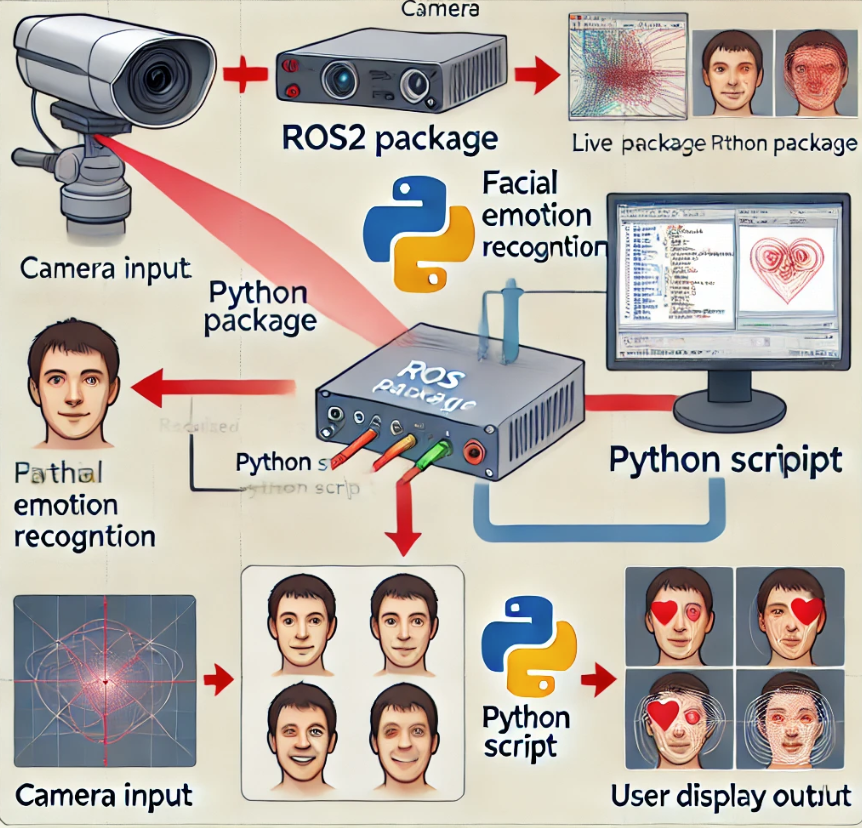
\includegraphics[width=0.8\textwidth]{img/connection.png}
    \caption{Schéma systému na rozpoznávanie emócií operátora pomocou RGB kamery.} 
    \label{fig:schema}
\end{figure}
\section{Teoretické základy}
\subsection{Emócie a ich prejav}
Emócie sú komplexné psychologické stavy, ktoré zahŕňajú subjektívne zážitky, fyziologické reakcie a behaviorálne prejavy. V priebehu výskumu boli emócie definované rôznymi spôsobmi, 
ale všeobecne sa považujú za reakcie na podnety, ktoré ovplyvňujú ľudské správanie a myslenie. Emócie môžu byť pozitívne alebo negatívne a ovplyvňujú naše rozhodovanie, pamäť a vnímanie sveta okolo nás. \cite{article01}
\subsubsection{Univerzálne emócie}
Jednou z najvýznamnejších teórií o emóciách je teória univerzálnych emócií, ktorú vyvinul psychológ Paul Ekman. Podľa tejto teórie existuje šesť základných emócií, ktoré sú univerzálne rozpoznateľné 
na základe výrazu tváre: radosť, smútok, hnev, prekvapenie, strach a odpor​. Tieto emócie sú nezávislé od kultúrnych vplyvov a prejavujú sa podobným spôsobom naprieč rôznymi kultúrami a etnickými skupinami. \cite{article03}
\subsubsection{Kultúrne rozdiely v prejave emócií}
Napriek existencii univerzálnych emócií existujú významné kultúrne rozdiely v tom, ako sú emócie prejavované a vnímané. Niektoré kultúry, ako napríklad západné, sú viac orientované na individualizmus, 
kde je prejav emócií otvorenejší a priamy, zatiaľ čo v kolektivistických kultúrach, ako sú východné ázijské krajiny, sú emócie častejšie potláčané alebo prejavované menej intenzívne​. \cite{article01}
\subsubsection{Výrazy tváre ako indikátory emócií}
Výraz tváre je jedným z hlavných spôsobov, ako sú emócie vonkajšie prejavované. Svalové pohyby tváre, ktoré zahŕňajú zmeny v oblasti očí, obočia, úst a líc, sú kľúčovými indikátormi emočných stavov. 
Tento typ neverbálnej komunikácie je extrémne efektívny, pretože umožňuje okamžitý a intuitívny prenos emocionálnych informácií​ \cite{inProceedings01}. Výskum ukázal, že až 55 \% emočných informácií je 
prenášaných prostredníctvom výrazov tváre, čo zdôrazňuje ich význam v sociálnej interakcii​. \cite{article03}
\subsection{Analýza obrazu}
Analýza obrazu je kľúčová pre proces rozpoznávania emócií na základe tváre. Tento proces zahŕňa detekciu tváre, extrakciu príznakov a následnú klasifikáciu emócií​
\subsubsection{Detekcia tváre}
Detekcia tváre je prvým krokom v procese rozpoznávania emócií. Tento krok zahŕňa lokalizáciu tváre v obraze a je rozhodujúci pre ďalšie spracovanie. Moderné metódy detekcie tváre, ako je algoritmus Viola-Jones,
 používajú rýchle a efektívne prístupy k lokalizácii tvárových oblastí, čo je nevyhnutné pre následné kroky​. Vývoj hlbokých neurónových sietí, ako sú konvolučné neurónové siete (CNN), výrazne zlepšil presnosť 
 detekcie tváre, čo umožnilo rozpoznávať tváre aj v rôznych svetelných podmienkach a uhloch​.\cite{article03}

\textbf{Metódy:}

Metóda Haar Cascade využíva sériu funkcií odvodených z Haar-like vzorov, ktoré sa používajú na identifikáciu oblastí záujmu. Tieto vzory umožňujú rýchlu detekciu, pričom proces je optimalizovaný pomocou 
"Integral Image". Napriek svojej robustnosti pri čelných záberoch sme identifikovali výzvy pri zmene osvetlenia a uhla záberu, ktoré sme riešili dodatočnou normalizáciou jasu a kontrastu.
Algoritmus využíva preddefinované Haar-like príznaky (ako vzory okienka pre kontrastné oblasti, napr. oči vs. líca). Používa koncept Integral Image, ktorý znižuje výpočtovú náročnosť výberu príznakov. 
Tréning klasifikátora sa vykonáva pomocou algoritmu AdaBoost, ktorý identifikuje najvýznamnejšie príznaky. Detekcia prebieha cez viacero "okienok" rôznej veľkosti na snímke.

Detekcia tváre pomocou face\_net (SSD model) využíva predtrénovaný model SSD (Single Shot MultiBox Detector) s architektúrou Caffe na detekciu tvárí. Táto metóda je modernejšia a 
efektívnejšia oproti Haar Cascade, pretože využíva hlboké neurónové siete na extrakciu robustných príznakov.
Princíp fungovania je optimalizovaný na detekciu viacerých objektov naraz, pričom predikcie sú vykonávané na rôznych úrovniach vrstiev CNN.Model využíva vstupnú veľkosť obrazu 300x300 pixelov a 
predspracovanie obrazu na odstránenie šumu (normalizácia s hodnotami RGB: 104.0, 177.0, 123.0). Výstup modelu obsahuje confidence score (pravdepodobnosť detekcie) a súradnice ohraničujúceho boxu.

\begin{figure}[!htpb]
    \centering
    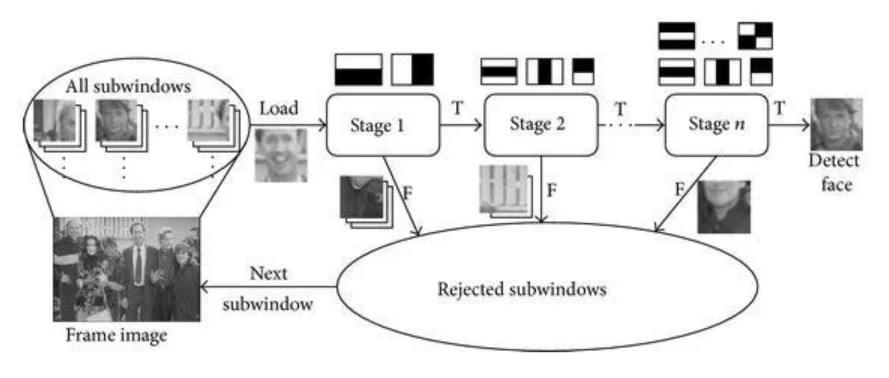
\includegraphics[width=0.8\textwidth]{img/haar_cascade.png}
    \caption{Detekcia tváre pomocou Haar Cascade.} 
    \label{fig:haar_cascade}
    % https://medium.com/@baselanaya/faces-detection-using-haar-cascade-3e175aef84f5
\end{figure}

\begin{figure}[!htpb]
    \centering
    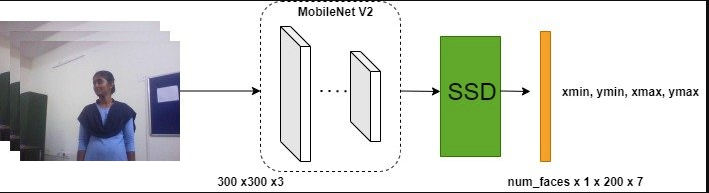
\includegraphics[width=0.8\textwidth]{img/ssd_model.png}
    \caption{Detekcia tváre pomocou SSD modelu.} 
    \label{fig:ssd_model}
    % https://www.researchgate.net/figure/Face-Detector-Model-MobilenetV2-ssd-head_fig2_345431258
\end{figure}
\subsubsection{Extrakcia príznakov}
\textbf{Toto dat asi jak podkapitotlu ku detekcii tvare pomocou CV a NN.}
Po detekcii tváre nasleduje extrakcia príznakov, kde sú identifikované kľúčové črty tváre, ako sú oči, nos, ústa a obočie. Tieto črty sú dôležité pre analýzu výrazov tváre, pretože zmeny v ich polohe 
alebo napätí súvisia s rôznymi emočnými stavmi​. \cite{inProceedings01} Typické algoritmy používané pri extrakcii príznakov zahŕňajú Gaborove filtre a histogramy orientovaných gradientov (HOG), 
ktoré zameriavajú pozornosť na zmeny v textúre a tvaroch​.\cite{article03}.
\subsubsection{Klasifikácia}
Klasifikácia emócií je záverečným krokom, kde sú extrahované príznaky spracované a priradené k určitým emočným kategóriám. Moderné metódy klasifikácie používajú algoritmy strojového učenia, 
ako sú Support Vector Machines (SVM), ale najúčinnejšie sú konvolučné neurónové siete (CNN), ktoré dokážu automaticky klasifikovať výrazy do kategórií, ako sú šťastie, smútok alebo hnev​. \cite{inProceedings01} \cite{article03}

\subsection{Biometria}
Biometria sa zaoberá rozpoznávaním osôb na základe jedinečných fyziologických alebo behaviorálnych charakteristík. V oblasti rozpoznávania tváre ide o identifikáciu alebo verifikáciu osôb 
na základe tvárových čŕt​. \cite{inProceedings01} \cite{article03}
\subsubsection{Princípy biometrických systémov}
Biometrické systémy sú založené na zhromažďovaní a analýze údajov, ktoré sú pre jednotlivca jedinečné, ako sú odtlačky prstov, dúhovka alebo tvár. Tieto systémy musia byť schopné spoľahlivo identifikovať 
alebo overiť osobu na základe týchto údajov. V kontexte rozpoznávania tváre systém spracováva obraz tváre, extrahuje relevantné črty a porovnáva ich s uloženými údajmi​. \cite{article01}
\subsubsection{Identifikácia vs. verifikácia}
Identifikácia a verifikácia sú dva hlavné prístupy v biometrických systémoch. Identifikácia zahŕňa určenie identity osoby na základe údajov o tvári v porovnaní s databázou, zatiaľ čo verifikácia porovnáva 
údaje jednej osoby s predtým zaznamenanými údajmi, aby potvrdila, či ide o tú istú osobu​\cite{inProceedings01}. Rozpoznávanie tváre je často používané v aplikáciách na bezpečnosť, kde verifikácia 
hrá kľúčovú úlohu pri autentifikácii používateľov, zatiaľ čo identifikácia sa používa na vyhľadávanie osôb v rozsiahlych databázach.\cite{article03}

\section{Existujúce metody analýzy emócií}
V oblasti rozpoznávania emócií na základe výrazu tváre existuje mnoho prístupov, ktoré môžeme rozdeliť na manuálne a automatizované metódy. Kým tradičné manuálne prístupy spočívajú v ručnom označovaní 
výrazov tváre, moderné metódy využívajú automatické algoritmy, často založené na neurónových sieťach (NN).

\subsection{Ručne značenie}
Ručne značenie (manuálna anotácia) spočíva v označovaní kľúčových bodov na tvári a následnom priradení výrazov tváre k určitým emočným kategóriám. Tento proces je časovo náročný a vyžaduje expertov 
na interpretáciu dát. Avšak, ručné značenie je stále dôležité pre tvorbu datasetov, ktoré sú nevyhnutné na trénovanie automatických systémov. Dôležité datasetové projekty, ako sú Cohn-Kanade alebo AffectNet, 
sa opierajú o ručné značenie výrazov tváre​. Manuálna anotácia má významnú úlohu v počiatočných fázach výskumu, ale pre aplikácie, ktoré vyžadujú veľké množstvo dát, je neefektívna. \cite{article01}

\subsection{Automatická analýza emócií}
Automatická analýza emócií využíva pokročilé algoritmy počítačového videnia a strojového učenia, aby bola schopná rozpoznať emócie na základe výrazu tváre bez potreby manuálneho zásahu. 
Moderné systémy rozpoznávania emócií sa vo veľkej miere spoliehajú na neurónové siete (NN), najmä na konvolučné neurónové siete (CNN), ktoré dokážu automaticky extrahovať a klasifikovať príznaky výrazu tváre.

\subsubsection{Konvolučné neurónové siete}
Neurónové siete sú inšpirované biologickými mozgovými štruktúrami a sú schopné učiť sa z obrovských množstiev dát. Pre úlohy rozpoznávania obrazu, vrátane rozpoznávania emócií, 
sú najbežnejšie využívané konvolučné neurónové siete (CNN)​. CNN majú schopnosť automaticky extrahovať črty tváre bez potreby manuálnej definície a v kombinácii s ďalšími typmi sietí,
ako sú rekurentné neurónové siete (RNN) alebo dlhodobé pamäte (LSTM), umožňujú ešte lepšiu interpretáciu časovo premenlivých dát, ako sú sekvencie výrazov tváre. \cite{article01} \cite{misc01}

\subsubsection{Typy vhodných neurónových sietí}
Pre aplikácie rozpoznávania emócií sa osvedčili rôzne typy neurónových sietí:

\textbf{Konvolučné neurónové siete (CNN):} CNN sa často používajú na extrakciu priestorových príznakov z obrazov tváre, ako sú oči, ústa a obočie​. CNN sú obzvlášť účinné pri identifikácii týchto príznakov 
z rôznych uhlov a svetelných podmienok. \cite{article05}

\textbf{Rekurentné neurónové siete (RNN) a LSTM: }Tieto siete sú vhodné pre analýzu sekvencií, ako sú videozáznamy alebo opakujúce sa výrazy tváre. Použitím týchto sietí je možné zohľadniť časové zmeny v tvári,
 čo je dôležité pre interpretáciu dynamických emócií​. \cite{article02}

\textbf{Deep Convolutional Neural Networks (DCNN): } DCNN je špeciálny typ CNN, ktorý dosahuje vysokú presnosť v úlohách rozpoznávania emócií, najmä pri kombinácii s technológiami počítačového videnia.
\subsubsection{Príklady použitia počítačového videnia}
ozpoznávanie emócií je úzko prepojené s oblasťou počítačového videnia. Počítačové videnie používa algoritmy na interpretáciu vizuálnych informácií. V súčasnosti sa CNN často kombinujú s technológiami, 
ako sú techniky extrakcie príznakov (napr. HOG alebo SIFT), aby sa zlepšila presnosť rozpoznávania výrazu tváre. Tieto systémy sú schopné identifikovať a klasifikovať tvárové príznaky aj v náročných podmienkach,
 ako sú premenlivé svetelné podmienky alebo čiastočné zakrytie tváre.\cite{Huang2023}


\section{Návrh riešenia}        %section 4
\subsection{Porovnanie vybraných metód}
V dokumente sa ako hlavné metódy použili kombinácia OpenCV a konvolučných neurónových sietí (CNN), pričom tieto technológie boli zvolené kvôli schopnosti riešiť výzvy 
spojené so zmenami osvetlenia, rôznymi pózami a potrebou rýchleho spracovania v reálnom čase. OpenCV slúžil na efektívne predspracovanie dát a 
detekciu tvárí pomocou Haar cascade classifier, zatiaľ čo CNN umožnili extrakciu komplexných čŕt a klasifikáciu emócií. Ako základ bola použitá predtrénovaná
architektúra VGGFace, ktorá výrazne zlepšila presnosť systému a skrátila čas potrebný na tréning. Model bol trénovaný na datasete FER2013, ktorý obsahoval obrázky
kategorizované podľa siedmich základných emócií (šťastie, smútok, hnev, prekvapenie, strach, znechutenie a neutrálne). Na optimalizáciu modelu bol použitý Adam 
algoritmus a cross-entropy loss funkcia. Výsledný systém dosiahol vysokú presnosť 95,2 \% a bol schopný spracovať dáta v reálnom čase pri rýchlosti 25 snímok
za sekundu na priemernej PC zostave. V porovnaní s tradičnými metódami, ako sú ručne vytvárané črty spojené so strojovým učením, sa tento prístup ukázal ako 
oveľa presnejší a robustnejší, čím ponúka široké možnosti využitia v oblastiach ako sociálna robotika, zdravotníctvo a interakcia človek-stroj.\cite{inProceedings02}

V experimentoch bol model testovaný na klasifikáciu emócií, pričom dosiahnuté výsledky ukázali rôznu úroveň presnosti pre jednotlivé emócie. 
Najvyššiu presnosť dosiahol model pri detekcii neutrálneho výrazu, a to 88,5 \%, čo je pripisované jasným črtám a minimálnej nejednoznačnosti tohto výrazu. 
Pre kategóriu šťastia bola presnosť 85,2 \%, pričom niektoré chyby mohli byť spôsobené vplyvom osvetlenia. Klasifikácia smútku dosiahla presnosť 82,7 \%, 
čo ukazuje, že model si poradí aj so subtílnymi črtami, ako sú klesnuté kútiky úst či slzy. Pri kategórii hnevu bola presnosť 79,4 \%, kde variácie intenzity emócie 
predstavovali výzvu.\cite{inProceedings02}

Pre emóciu prekvapenia dosiahol model presnosť 77,1 \%, avšak jej prechodná povaha a možná podobnosť s inými emóciami spôsobovali ťažkosti. Najnižšiu presnosť 
model vykazoval pri kategóriách strachu (74,8 \%) a znechutenia, ktoré sú charakteristické jemnými a komplexnými výrazmi tváre. Tieto výsledky naznačujú,
že model je veľmi efektívny pri detekcii výrazných emócií, no u jemnejších a zriedkavejších prejavov si vyžaduje ďalšiu optimalizáciu. \cite{inProceedings02}
\begin{figure}[!htpb]
    \centering
    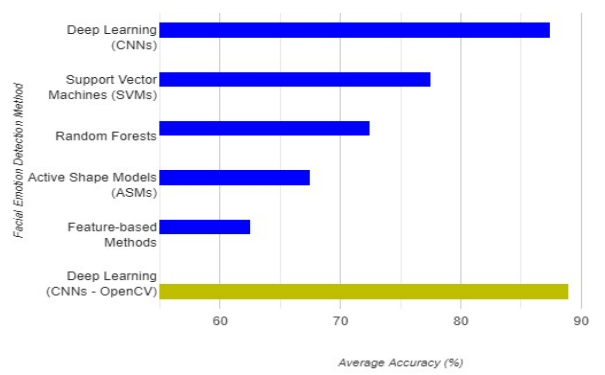
\includegraphics[width=0.8\textwidth]{img/comparation.png}
    \caption{porovnanie rôznych metód na rozpoznávanie emócií. \cite{inProceedings02}}
    \label{fig:comparation}
\end{figure}
\newpage
\subsection{Architektúra systému}
\begin{figure}[!htpb]
    \centering
    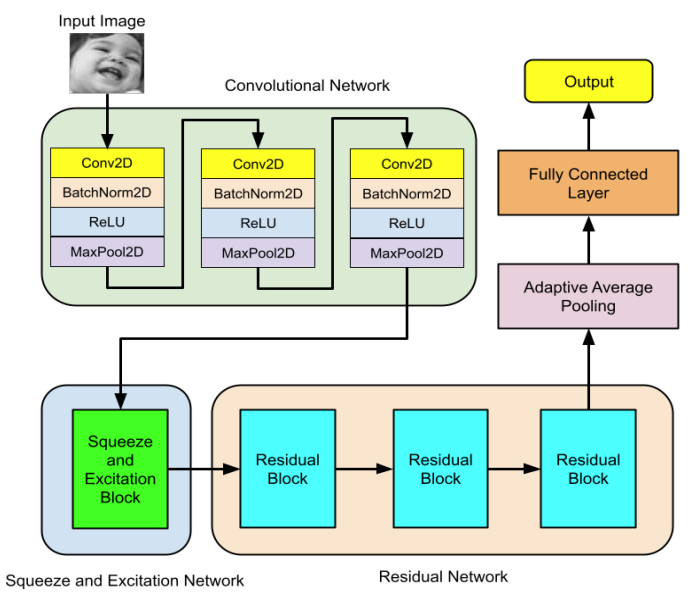
\includegraphics[width=0.8\textwidth]{img/architecture.png}
    \caption{Architektúra systému na rozpoznávanie emócií operátora pomocou RGB kamery.} 
    \label{fig:architecture}
\end{figure}
\newpage

\subsection{Výber dát}
Dataset FER2013 (Facial Expression Recognition 2013) je jedným z najčastejšie používaných datasetov na trénovanie a testovanie modelov na rozpoznávanie emócií. 
Obsahuje 35 887 obrázkov v odtieňoch sivej, pričom každý má rozlíšenie 48x48 pixelov. Obrázky sú kategorizované do siedmich emócií: šťastie, smútok, hnev, 
prekvapenie, strach, znechutenie a neutrálne. Dataset je rozdelený na trénovaciu, validačnú a testovaciu časť, čo umožňuje komplexné testovanie a optimalizáciu 
modelov. Najviac obrázkov obsahuje kategória „šťastie“, zatiaľ čo kategória „znechutenie“ má najmenej obrázkov, čo vedie k nerovnomernému rozloženiu dát medzi 
triedami. \newline
\textbf{Ďalšie podobné datasety}
\begin{itemize}
    \item \textbf{AffectNet:} Obsahuje viac ako 1 milión obrázkov, ktoré sú anotované na 11 kategórií emócií vrátane neutrálnych a jemných variácií ako „záujem“ či „zvedavosť“.
    \item \textbf{CK+ (Cohn-Kanade Extended):} Obsahuje 593 sekvencií tvárových výrazov, ktoré pokrývajú 7 základných emócií. Obrázky sú vysokej kvality a často sa používajú na analýzu prechodov medzi neutrálnymi a výrazovými stavmi.
    \item \textbf{KDEF (Karolinska Directed Emotional Faces): }Obsahuje 4900 obrázkov od 70 jedincov, pričom každý jedinec zobrazuje 7 emócií. Je špecificky navrhnutý na psychologické experimenty a rozpoznávanie emócií.
    \item \textbf{EmoReact: }Dataset určený na rozpoznávanie emócií z videí, obsahuje multimodálne dáta vrátane audio a vizuálnych záznamov. Je užitočný pri štúdiu komplexnejších interakcií medzi emóciami a dynamickými prejavmi.
\end{itemize}
Datasety ako FER2013 a AffectNet sú preferované pre svoju veľkosť a rozmanitosť, zatiaľ čo menšie datasety ako JAFFE a CK+ sa často používajú na overenie 
základných hypotéz a pilotné štúdie. Výber datasetu závisí od konkrétneho cieľa výskumu a požiadaviek na presnosť a robustnosť modelu.

\subsection{Extrakcia príznakov}

Extrakcia príznakov je kľúčovým krokom v procese analýzy tvárových emócií, pretože umožňuje modelu identifikovať a rozpoznať črty tváre, 
ktoré súvisia s konkrétnymi emóciami. Tento proces sa zvyčajne skladá z niekoľkých fáz, ktoré sú založené na kombinácii počítačového videnia a 
metód strojového učenia:
\begin{enumerate}
    \item \textbf{Predspracovanie obrazu:} Pred extrakciou sa obraz upravuje na zjednodušenie analýzy: 
    \begin{itemize}
        \item \textbf{Normalizácia:} Normalizácia farieb a kontrastu na zjednotenie vlastností obrazu.
        \item \textbf{Orezanie:} Odstránenie okrajov a pozadia, aby sa zvýraznili relevantné časti tváre.
        \item \textbf{Zmena veľkosti:} Zmena rozlíšenia obrazu na zjednotenie veľkosti vstupov.
    \end{itemize}
    \item \textbf{Detekcia kľúčových bodov tváre: } V tejto fáze sa identifikujú charakteristické body tváre, ako sú oči, nos, ústa a obočie: 
    \begin{itemize}
        \item \textbf{Algoritmy detekcie:} Bežne sa používajú metódy ako Haar Cascade, Dlib, MTCNN, OpenPose, SSD model. Tieto metódy poskytujú presné súradnice bodov tváre, ktoré sú základom na analýzu zmien v jednotlivých oblastiach.
    \end{itemize}
    \item \textbf{Extrakcia príznakov:} Geometrické črty sa zameriavajú na vzdialenosti, uhly a proporcie medzi rôznymi bodmi na tvári. Tieto črty sú často použité na identifikáciu rozdielov medzi neutrálnymi a emocionálnymi výrazmi.
    \item \textbf{Použitie textúrových vlastností: } Textúrové vlastnosti poskytujú detailnejšie informácie o štruktúre tváre. Často sa využívajú metódy ako Gaborove filtre, HOG alebo LBP na extrakciu textúrnych príznakov.
    \item \textbf{Využitie konvolučných neurónových sietí (CNN): }Moderné prístupy nahrádzajú manuálnu extrakciu čŕt konvolučnými neurónovými sieťami:  
    \begin{itemize}
        \item \textbf{Konvolučné vrstvy:}  Automaticky detegujú a extrahujú črty relevantné pre konkrétne úlohy.
        \item \textbf{Pooling vrstvy:} Znižujú rozmer vstupov a zvyšujú invariantnosť voči posunom a zmenám veľkosti.
        \item \textbf{ReLU aktivačné funkcie:} Zvyšujú nelinearitu a umožňujú modelu učiť sa zložitejšie vzory.
        \item \textbf{Úplne prepojené vrstvy:} Kombinujú extrahované príznaky a klasifikujú ich do konkrétnych kategórií.
    \end{itemize}
    \item \textbf{Tvorba príznakového vektora:} Všetky extrahované črty (geometrické, textúrové, výstupy CNN) sa kombinujú do vysokodimenzionálneho vektora, ktorý reprezentuje obraz tváre. Tento vektor je vstupom pre klasifikátor (napr. Softmax, SVM), ktorý priradí tvár k jednej z kategórií emócií.
\end{enumerate}
Extrakované črty sú základom na rozpoznávanie jemných rozdielov medzi emóciami, ako napríklad zmena polohy obočia môže naznačovať hnev, zatiaľ čo stlačenie pier 
môže naznačovať smútok. Kombinácia čŕt a textúr umožňuje modelu pochopiť komplexné výrazy a správne ich kategorizovať. Táto postupnosť krokov zaisťuje, že model má prístup k najrelevantnejším informáciám z obrazu, čo zvyšuje presnosť klasifikácie emócií.

\subsection{Klasifikácia}
\subsection{Vyber hyperparametrov}

\section{Implementácia riešenia}
\subsection{Výber nástrojov}Programovací jazyk, knižnice (OpenCV, TensorFlow, PyTorch).
\subsection{Implementácia jednotlivých komponentov}Podrobný popis implementácie.
\subsection{Vizualizácia výsledkov}Vizualizácia výsledkov analýzy. Grafy, tabuľky.

\section{Implementácia v ROS2}
\subsection{Konverzia modelu}Konverzia trénovaného modelu do formátu vhodného pre ROS2.
\subsection{Integrácia do robotického systému}Popis integrácie do ROS2, komunikácia s ostatnými modulmi.

\section{Exprerimenty a vyhodnotenie}
\subsection{Dátová sada} Popis použitého dataset-u (veľkosť, rozdelenie tried, kvalita).
\subsection{Metriky} Výber vhodných metrik (presnosť, úplnosť, F1-skóre, ROC krivka).
\begin{figure}[!htpb]
    \centering
    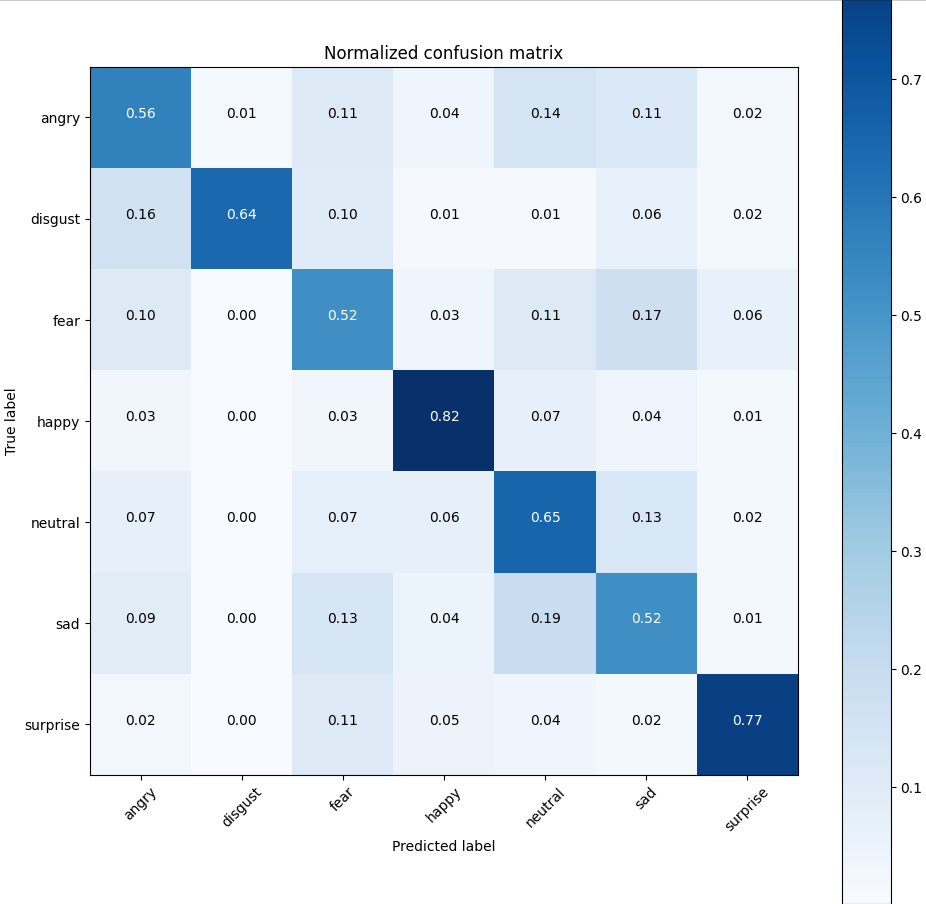
\includegraphics[width=0.8\textwidth]{img/confusion.png}
    \caption{Confusion matrix.}
    \label{fig:confusion}
\end{figure}
\begin{figure}[!htpb]
    \centering
    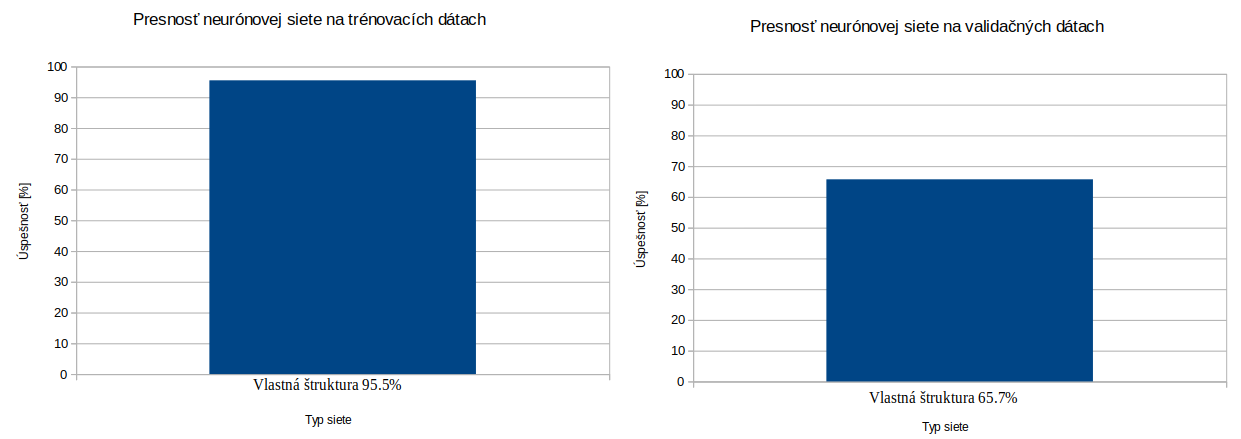
\includegraphics[width=0.8\textwidth]{img/train_graphs.png}
    \caption{Trénovacie grafy.}
    \label{fig:roc}
\end{figure}
\newpage

\subsection{Výsledky} Vyhodnotenie výsledkov experimentov. Prehľadné zhrnutie výsledkov, porovnanie s inými prácami.
\begin{figure}[!htpb]
    \centering
    \begin{subfigure}[b]{0.45\textwidth}
        \centering
        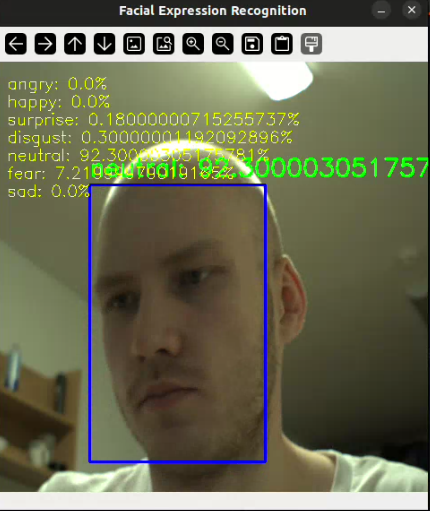
\includegraphics[width=\textwidth]{img/neutral.png}
        \caption{Neutral}
        \label{fig:neutral}
    \end{subfigure}
    \hfill
    \begin{subfigure}[b]{0.45\textwidth}
        \centering
        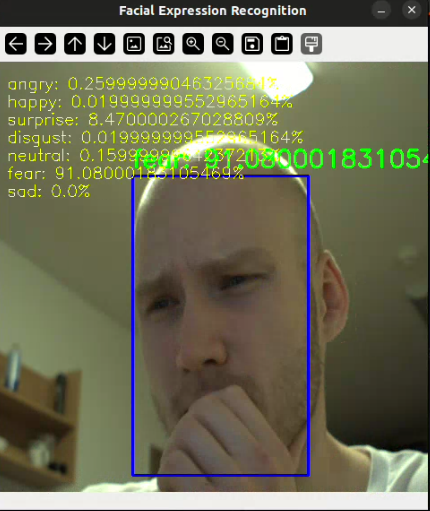
\includegraphics[width=\textwidth]{img/fear.png}
        \caption{Fear}
        \label{fig:fear}
    \end{subfigure}
    \vskip\baselineskip
    \begin{subfigure}[b]{0.45\textwidth}
        \centering
        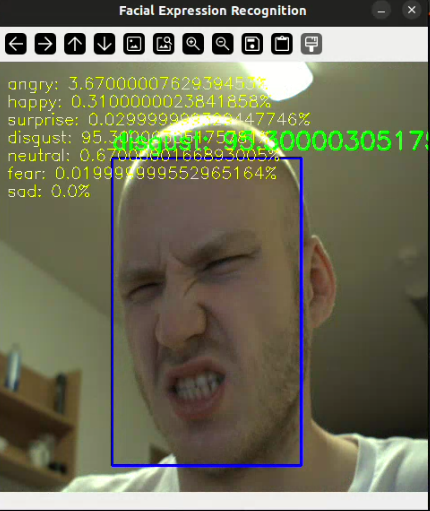
\includegraphics[width=\textwidth]{img/disgust.png}
        \caption{Disgust}
        \label{fig:disgust}
    \end{subfigure}
    \hfill
    \begin{subfigure}[b]{0.45\textwidth}
        \centering
        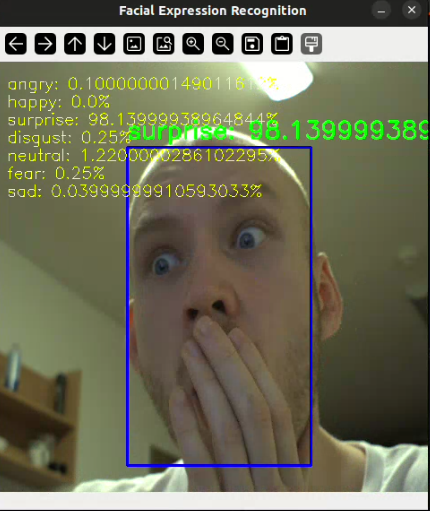
\includegraphics[width=\textwidth]{img/surprise.png}
        \caption{Surprise}
        \label{fig:surprise}
    \end{subfigure}
    \caption{Examples of different facial expressions.}
    \label{fig:expressions}
\end{figure}
\newpage
\subsection{Analýza výsledkov} Analýza výsledkov, príčiny chýb, možné zlepšenia.


\section{Záver}
\subsection{Zhodnotenie práce}Zhodnotenie dosiahnutých výsledkov.
\subsection{Obmedzenia práce}Obmedzenia práce, možné zlepšenia.
\subsection{Budúce smerovanie}Možné smerovanie ďalšej práce.

\section{Doplnujece poznamky }
Literatúra: Pravidelne citujte relevantnú literatúru.
Obrázky a diagramy: Používajte obrázky a diagramy na ilustráciu komplexných konceptov.
Kód: Ak je to možné, pridajte ukážky kódu.
Tabuľky: Používajte tabuľky na porovnanie výsledkov.
Táto štruktúra poskytuje komplexný rámec pre vašu prácu. Môžete ju prispôsobiť podľa svojich konkrétnych potrieb a zistení.
\section{Plán práce na ďalši semester}
\begin{itemize}
    \item Implementácia iné štruktúry neuronovej siete pre dosiahnutie lepších výsledkov.
    \item Testovanie systému na simulovaných a reálnych dátach.
    \item Integrácia systému do robotických platforiem.
    \item Experimenty a vyhodnotenie výsledkov.
    \item Napísanie záverečnej práce.
    \item Obhajoba záverečnej práce.
\end{itemize}